\documentclass[a4paper,11pt]{jsarticle}


% 数式
\usepackage{amsmath,amsfonts}
\usepackage{bm}
\usepackage{physics}
% 画像
\usepackage[dvipdfmx]{graphicx}
% ローマ数字
\usepackage{otf}
% 単位
\usepackage{siunitx}
% 表
\usepackage{multirow}
% 化学反応
\usepackage[version=4]{mhchem}

\begin{document}

\title{理論演習 ゴミ分子の導入}
\author{齋藤駿一}
\date{\today 編集}
\maketitle

\section{概要}

まず,ゴミ分子(と複合体)の存在が成長速度に与える影響を明確にしようとしたが,うまくいかなかった.
そこで,反応ネットを最小($N=2$)にした上で,複合体が分解する場合としない場合で,栄養濃度と成長速度の関係,および栄養濃度と膜のゴミ分子の濃度の関係がどう変わるかを調べた.
その結果から,複合体の分解によって,低濃度側では成長速度の低下が抑えられ,高濃度側では反応ネットワークによる多様性が生まれるのではないかと考えた.
ただし,エラー率1で成長が見られるため,プログラムにミスがある可能性もある.

\section{ゴミ分子の影響}
初期値は,活性のある分子については1,ゴミ分子と複合体については0とした.

まず,栄養濃度を$n=1$と固定して,connection rate $p=0.2,0.8$についてエラー率と成長速度の関係を調べたところ,それぞれ図\ref{fig:eg_p02}および図\ref{fig:eg_p08}のようになった\footnote{当初は各エラー率のもとで生成した反応ネットの間で成長速度の平均値をとるつもりだったが,あまりにも誤差が大きいのでやめた.}.
この結果から,どのエラー率でも成長速度の小さい反応ネットワークは現れうるが,成長速度の分布(とくに上限のようなもの)には制約がありそうだと分かった.
より正確な議論のためには,生成するランダム反応ネットの数を増やすか,それらの間で進化をさせる必要があると考える.

\begin{figure}[htbp]
  \centering
  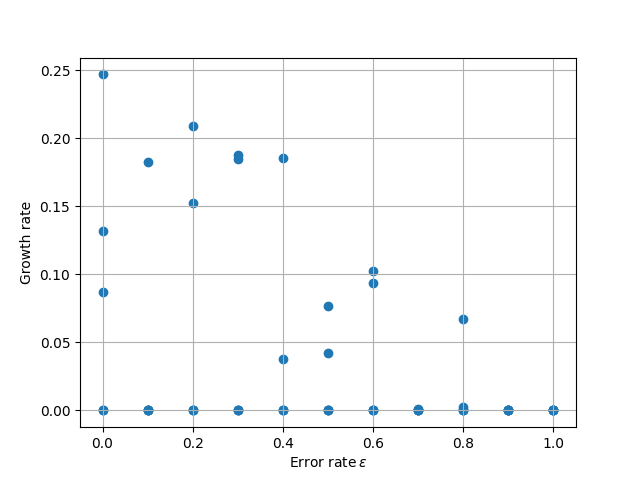
\includegraphics[width=10cm]{error_rate_growth_rate_N5_T5_p02_2.png}
  \caption{$p=0.2$のときのエラー率と成長速度の関係.各エラー率に対し5通りのランダムネットを作って計算した.}
  \label{fig:eg_p02}
\end{figure}

\begin{figure}[htbp]
  \centering
  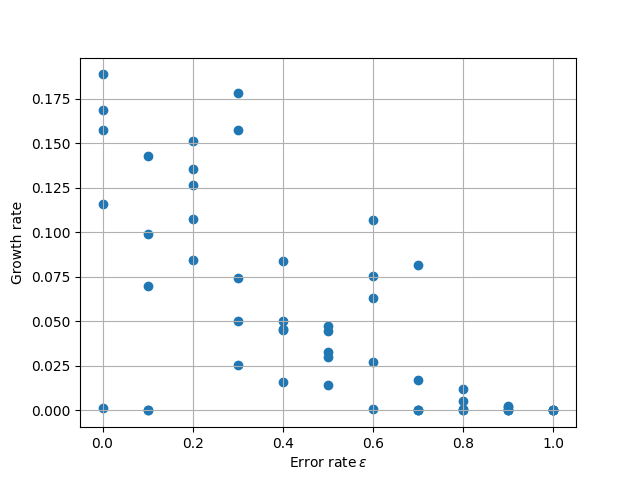
\includegraphics[width=10cm]{error_rate_growth_rate_N5_T5_p08_2.png}
  \caption{$p=0.8$のときのエラー率と成長速度の関係.各エラー率に対し5通りのランダムネットを作って計算した.}
  \label{fig:eg_p08}
\end{figure}

また,前回のプログラムで制限時間を$T=10^3$から$T=10^5$に延ばして計算したところ,栄養濃度と成長速度の関係は図\ref{fig:ng_p08}のようになった.
前回と「転移点」がずれているので,やはり前回の「転移」は制限時間による見せかけのものだった可能性が高い.
一方で,高栄養濃度に注目すると,$n=1$前後でゆるい転移が見られた.
しかし,これはエラー率0でも見られた(図\ref{fig:ng_p08_err0})ので,ゴミ分子によるものではないと分かった.

\begin{figure}[htbp]
  \centering
  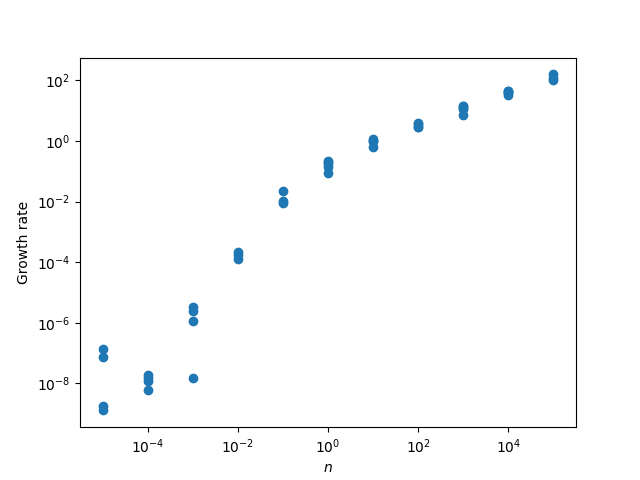
\includegraphics[width=10cm]{waste_N5_T5_p08_4.png}
  \caption{エラー率$\epsilon=0.001$,connection rate $p=0.8$のときの栄養濃度と成長速度の関係.各栄養濃度に対し5通りのランダムネットを作って計算した.}
  \label{fig:ng_p08}
\end{figure}

\begin{figure}[htbp]
  \centering
  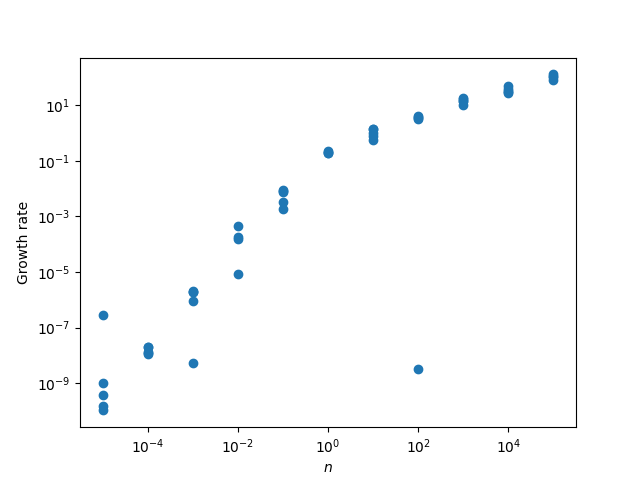
\includegraphics[width=10cm]{waste_N5_T5_p08_err0.png}
  \caption{エラー率$\epsilon=0$,connection rate $p=0.8$のときの栄養濃度と成長速度の関係.各栄養濃度に対し5通りのランダムネットを作って計算した.}
  \label{fig:ng_p08_err0}
\end{figure}

このことから,反応にネットワークがあるとゴミ分子が寄与する効果は小さいのかもしれないと考え,エラー率を0と0.5にとって比較したところ,挙動はほぼ変わらなかった(図\ref{fig:ng_p08_err0-05}).
結局,この段階ではゴミ分子の栄養を明確に確認することはできなかった.

\begin{figure}[htbp]
  \centering
  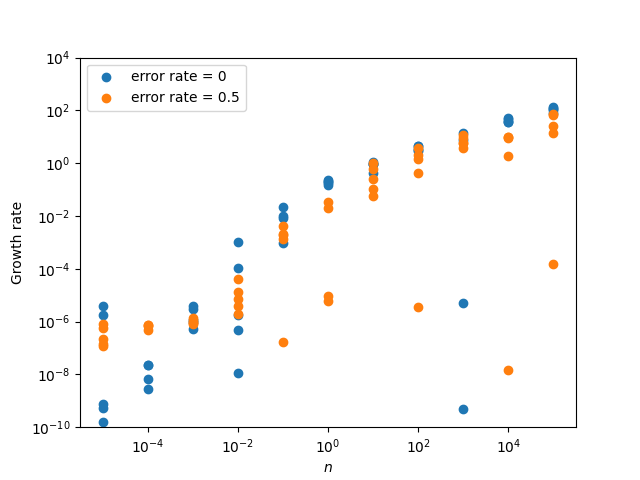
\includegraphics[width=10cm]{waste_N5_T5_p08_err.png}
  \caption{エラー率$\epsilon=0,0.5$,connection rate $p=0.8$のときの栄養濃度と成長速度の関係.各栄養濃度に対し5通りのランダムネットを作って計算した.}
  \label{fig:ng_p08_err0-05}
\end{figure}

また,プログラムが本当に正しいかのチェックも兼ねて,エラー率と栄養濃度を変えて,膜成分のゴミ分子の濃度をプロットすると,図\ref{fig:nwom_p08_err}のようになった.
ここでも,$n=1$を境に挙動が変わっているようだった.

\begin{figure}[htbp]
  \centering
  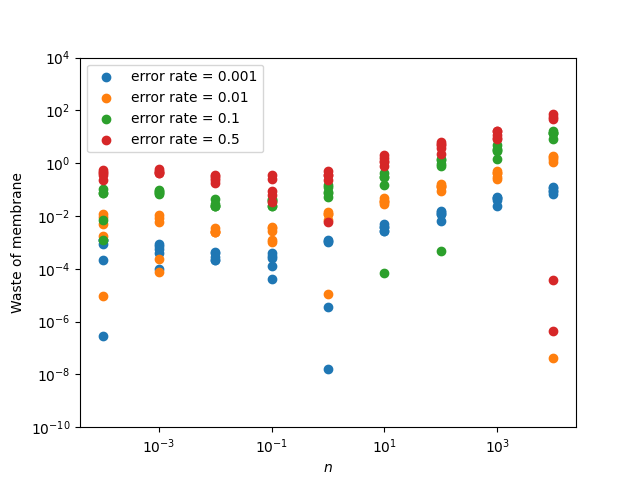
\includegraphics[width=10cm]{waste_N5_T5_p08_err_wom.png}
  \caption{栄養濃度と膜成分のゴミ分子の濃度の間の関係.ここには記していないが,エラー率0のとき,ゴミ分子の濃度はどの栄養濃度でも0になることを確認した.}
  \label{fig:nwom_p08_err}
\end{figure}

\section{パラメータの取り直し・複合体分解の意義}
以上のシミュレーションを経て,結局ゴミ分子を導入したことのありがたみが分からなくなった.
そこで,一度成分数を最小の$N=2$まで減らし\footnote{つまり栄養分子と膜分子しかない.},ゴミ分子から複合体ができる反応の速度定数を$\epsilon_p=1$と大きめに取り直した.
そして,逆に複合体が分解する反応の速度定数を$\epsilon_m=0,10^{-4}$の2通り考え,その間で比較することで,複合体分解の意義を考察した.

まず,栄養濃度と成長速度の関係は,$\epsilon_m=0$のとき図\ref{fig:ep1_em0_ng},$\epsilon_m=10^{-4}$のとき図\ref{fig:ep1_em04_ng}のようになった.
また,栄養濃度と膜のゴミ分子の濃度の関係は,$\epsilon_m=0$のとき図\ref{fig:ep1_em0},$\epsilon_m=10^{-4}$のとき図\ref{fig:ep1_em04}のようになった.
これらの図から,$\epsilon_m$の存在により,低濃度側では成長率の低下が抑えられ,高濃度側では反応ネットによって異なる挙動が生まれることが読み取れる.
しかし,$\epsilon_m=10^{-4}$のとき,エラー率1でも成長速度が0でないという点が奇妙であり,現在プログラムを見直している.

\begin{figure}[htbp]
  \centering
  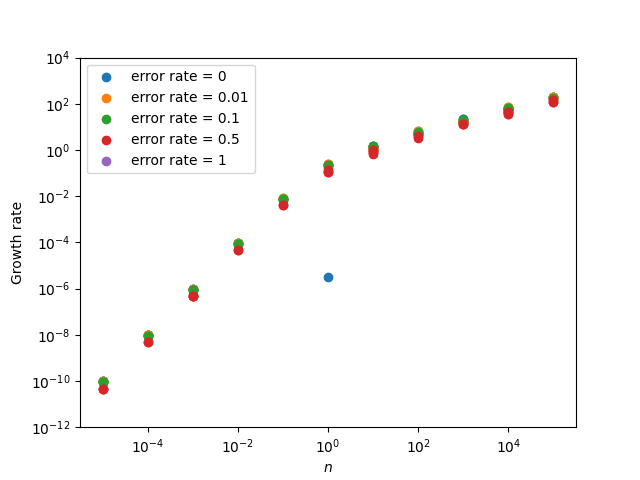
\includegraphics[width=10cm]{waste_N2_T5_p08_ep1_em0_ng.png}
  \caption{$N=2,p=0.8,\epsilon_p = 1, \epsilon_m = 0$とした場合の栄養濃度と成長速度の関係.}
  \label{fig:ep1_em0_ng}
\end{figure}

\begin{figure}[htbp]
  \centering
  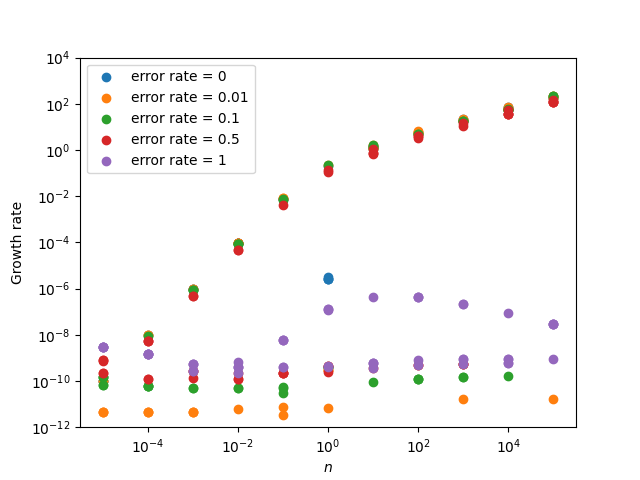
\includegraphics[width=10cm]{waste_N2_T5_p08_ep1_em4_ng.png}
  \caption{$N=2,p=0.8,\epsilon_p = 1, \epsilon_m = 10^{-4}$とした場合の栄養濃度と成長速度の関係.}
  \label{fig:ep1_em04_ng}
\end{figure}

\begin{figure}[htbp]
  \centering
  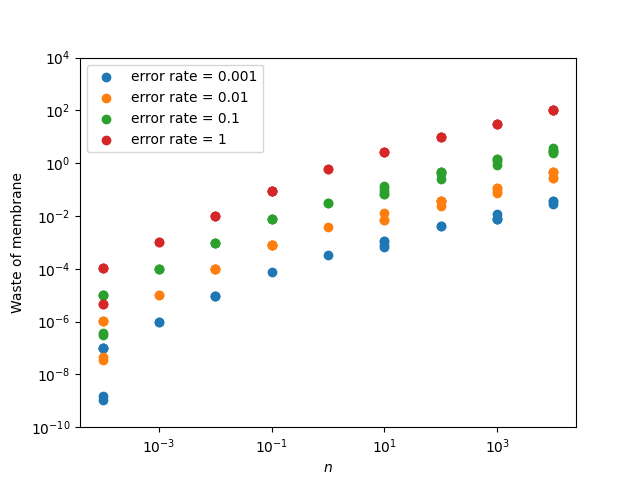
\includegraphics[width=10cm]{waste_N2_T5_p08_ep1_em0.png}
  \caption{$N=2,p=0.8,\epsilon_p = 1, \epsilon_m = 0$とした場合の栄養濃度と膜成分のゴミ分子の濃度の関係.}
  \label{fig:ep1_em0}
\end{figure}

\begin{figure}[htbp]
  \centering
  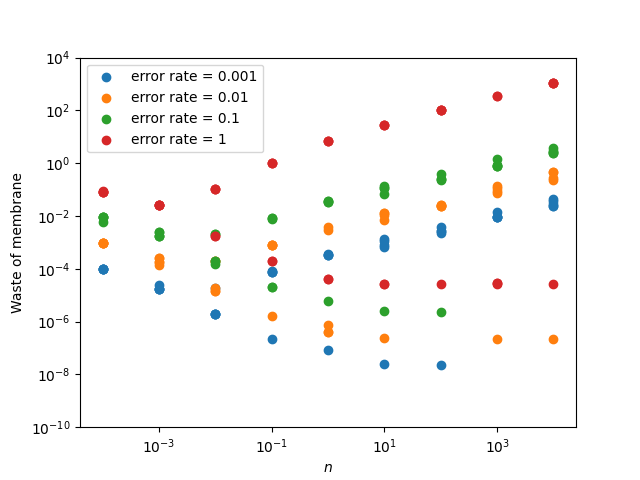
\includegraphics[width=10cm]{waste_N2_T5_p08_ep1_em4.png}
  \caption{$N=2,p=0.8,\epsilon_p = 1, \epsilon_m = 10^{-4}$とした場合の栄養濃度と膜成分のゴミ分子の濃度の関係.}
  \label{fig:ep1_em04}
\end{figure}

\end{document}